\documentclass[../main.tex]{subfiles}

\graphicspath{{../images/}}

\usepackage[noend]{algpseudocode} % for pseudocode
\usepackage[plain]{algorithm} % float environment for algorithms
% preferred pseudocode style
\algrenewcommand{\algorithmicprocedure}{}
\algrenewcommand{\algorithmicthen}{}

% ``do { ... } while (cond)''
\algdef{SE}[DOWHILE]{Do}{doWhile}{\algorithmicdo}[1]{\algorithmicwhile\ #1}%

% ``for (x in y ... z)''
\newcommand{\ForRange}[3]{\For{#1 \textbf{in} #2 \ \ldots \ #3}}

\begin{document}
\pagestyle{fancy}
\chead{Module 10}
\rhead{Junseo Shin}
\lhead{CSE 4059}


\renewcommand{\thefigure}{\arabic{figure}}
\section*{List Scan}

\subsection*{Questions}

\begin{enumerate}
    \item 3 Applications of parallel scan:
    \begin{enumerate}
        \item Radix sort or counting sorting
        \item Summed area table (SAT) for image processing (e.g. depth of field blurring)
        \item numerical integration (e.g. trapezoidal rule or Simpson's rule)
    \end{enumerate}

    \item There are 
    \begin{align*}
        N/2 + N/4 + \ldots + 1 = N - 1
    \end{align*}
    $n - 1$ additions in the up-sweep phase and 
    \begin{align*}
        \sum_{i = 1}^{\log_2{n}} \frac{n}{2^i} - 1 = n - 1 - \log_2{n}
    \end{align*}
    $n - 1 - \log_2{n}$ additions in the
    down-sweep phase for a total of $2n - 2 - \log_2{n}$ additions.
 
    \item The kernel has $2 \times \texttt{blockDim.x}$ global reads for the shared
    memory step since each thread reads 2 elements. So we have
    $2 \times \texttt{blockDim.x} \times \texttt{numBlocks}$ global reads.

    \item Just like the global reads, the writes are done once per block so we have
    $2 \times \texttt{blockDim.x} \times \texttt{numBlocks}$ global writes.

    \item MAX: A thread (the first thread) would have at max
    $2 \times \log_2{N} - 1$ additions in total ($\log_2{N} - 1$ per phase).

    MIN: A thread (the last) would have at min 1 addition in the up-sweep phase and
    0 additions in the down-sweep phase or 1 addition in total.

    AVERAGE: The average number of operations is then
    \begin{align*}
        \frac{2 \times \log_2{N} - 2 + 1}{N}
    \end{align*}

    \item In the up-sweep the stride doubles from 1 to $512$ or $\log_2{512} + 1= 10$ times, and 
    in the down-sweep the stride halves from $512/2 = 256$ to 1 or $\log_2{256} + 1 = 9$ times and
    once again after the last iterations so we have $10 + 9 + 1 = 20$ synchronizations in total
    for a block size of 512.

    \item We used shared memory to reduce the number of global memory accesses and also stored
    the sum of the block in the same kernel to reduce the number of kernel launches. Also


    \item We can implement thread coarsening and a single pass-scan (doing the segemented scan all
    in one kernel) to reduce the memory accesses.

    \item We have implemented a recursive segemented scan algorithm to handle
    an arbitrary number of elements! (it works with smaller block sizes up to dataset 12
    but 13 has some floating point errors propogating)

    \item if the order matters, we can use the Kogge-Stone scan algorithm for non-commutative
    operations.

    \item We can get different results because of the floating point errors that are non-associative.
\end{enumerate}

\newpage
\subsection*{OUPUT}
\begin{figure*}[ht]
    \centering
    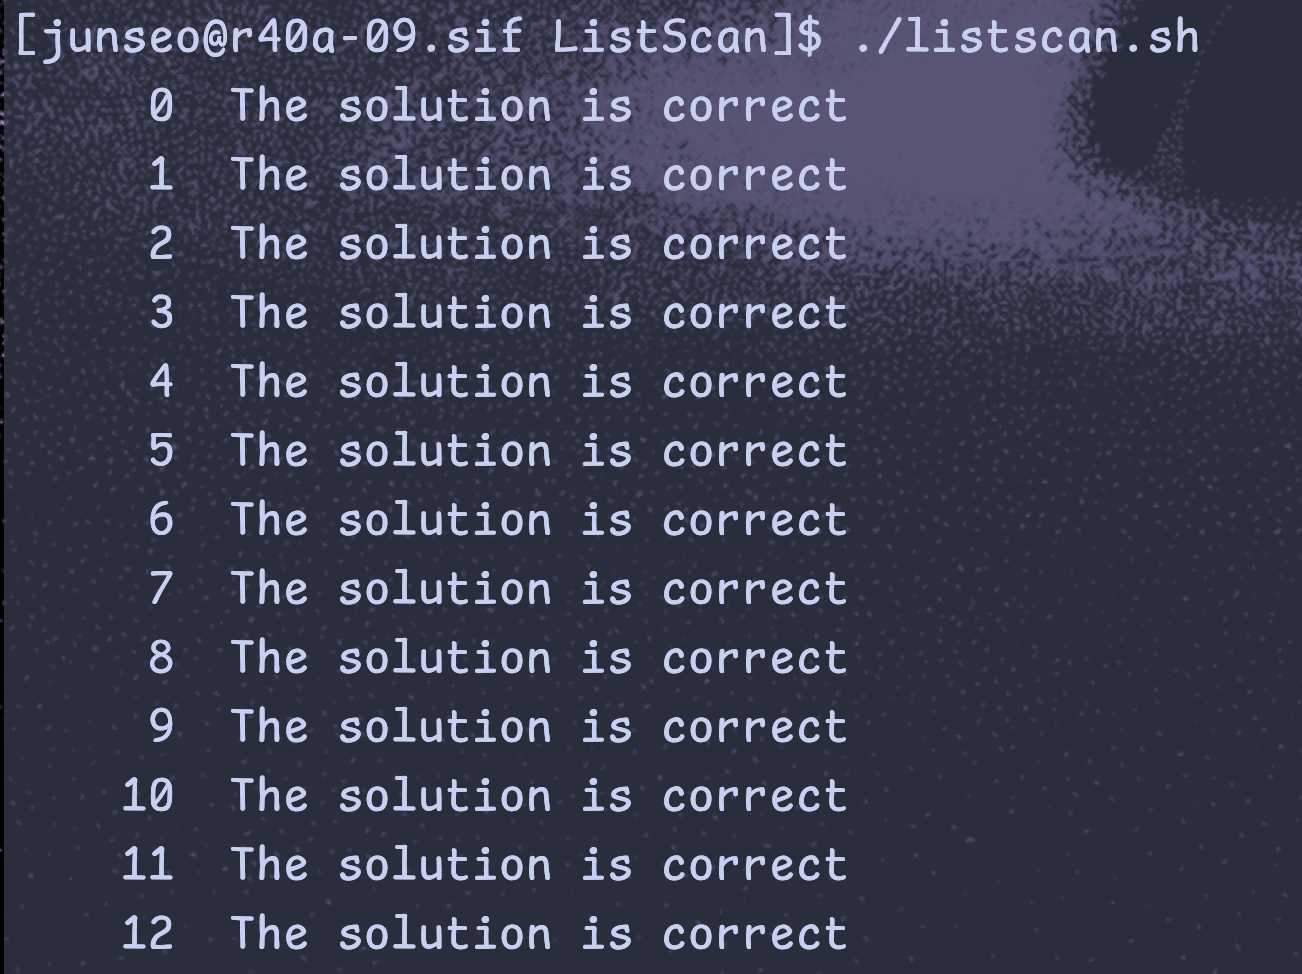
\includegraphics[width=0.8\textwidth]{listscan.png}
    \caption{Successes}
    \label{fig:listscan}
\end{figure*}

\end{document} 